\smallframetitle

\section{From 08/07/24 to 12/07/24}
\insertsectionframe

\subsection{further advancement on road detection}
\insertsubsectionframe

\begin{frame}{Cities and big cities connection graph}
    \begin{figure}
        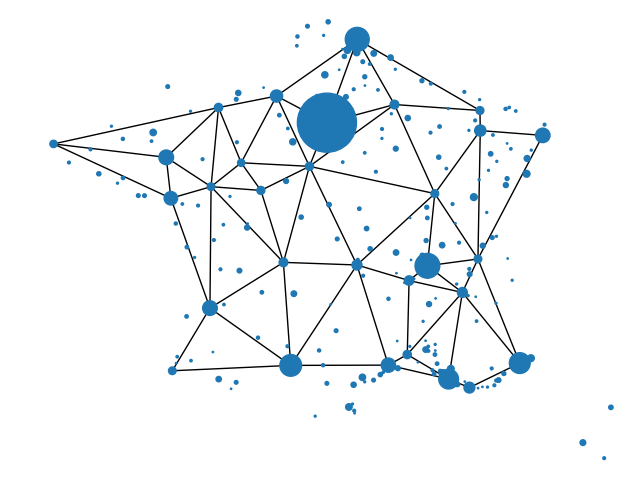
\includegraphics[height=0.6\paperheight]{images/road_detection/city_links_graph_all_cities.png}
        \caption{cities and big cities connection graph}
    \end{figure}
\end{frame}

\begin{frame}{Little cities linking method}
    \begin{block}{Steps}
        \begin{itemize}
            \item For each edge of the connection graph ;
            \item Detect all little cities close enough to this edge ;
            \item Create multiple edges to link all these cities together by a path with the same start and ending city than the big edge ;
        \end{itemize}
    \end{block}
    \begin{columns}
        \begin{column}{0.5\paperwidth}
            \begin{figure}
                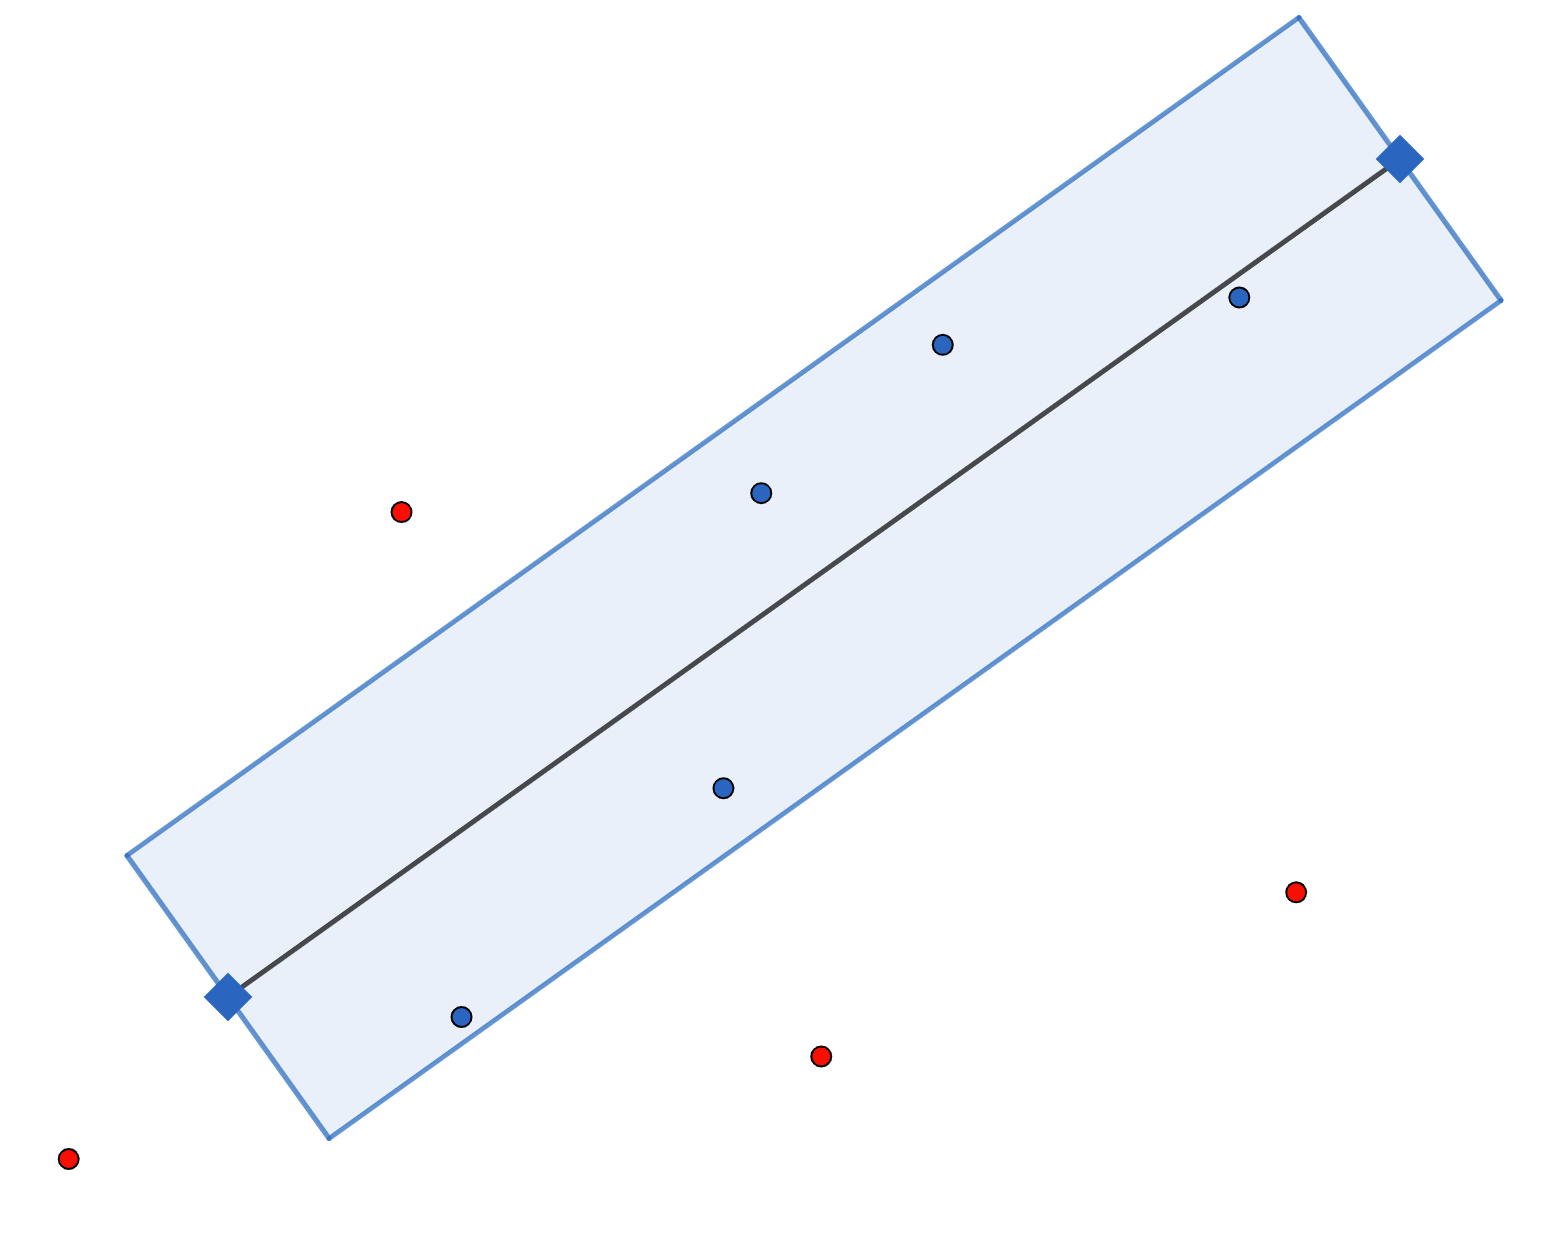
\includegraphics[height=0.3\paperheight]{images/road_detection/illustartion_city_selections.png}
                \caption{Little cities selection}
            \end{figure}
        \end{column}
        
        \begin{column}{0.5\paperwidth}
            \begin{figure}
                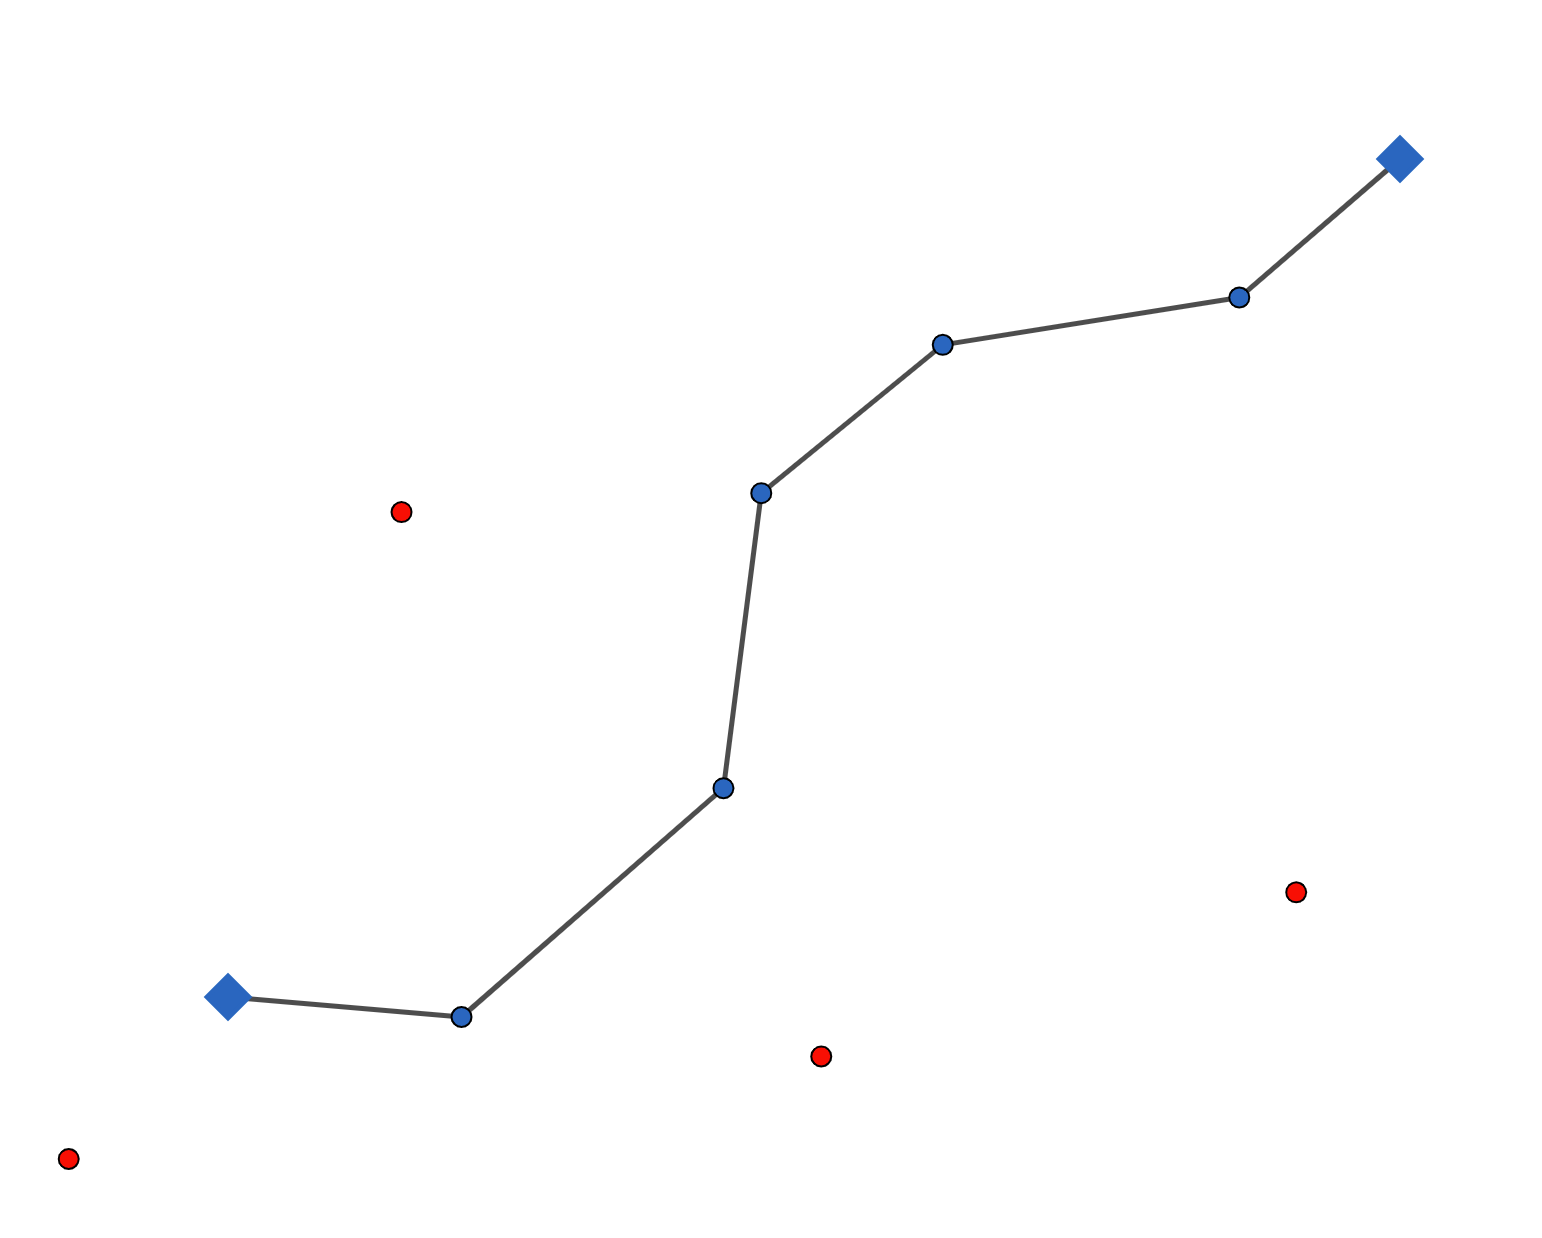
\includegraphics[height=0.3\paperheight]{images/road_detection/illustration_city_linkage.png}
                \caption{Cities linkage}
            \end{figure}
        \end{column}
    \end{columns}
\end{frame}

\begin{frame}{New graph after little city linkage}
    \begin{figure}
        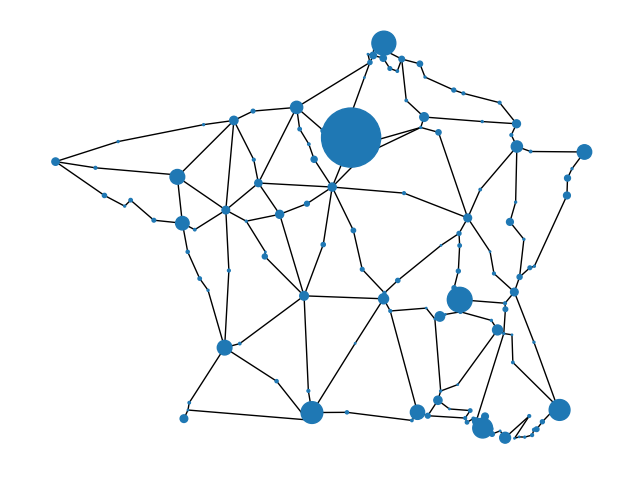
\includegraphics[height=0.6\paperheight]{images/road_detection/final_graph.png}
        \caption{Final graph (width parameter = $0.2$)}
    \end{figure}
\end{frame}

\begin{frame}{New graph on a map}
    \begin{figure}
        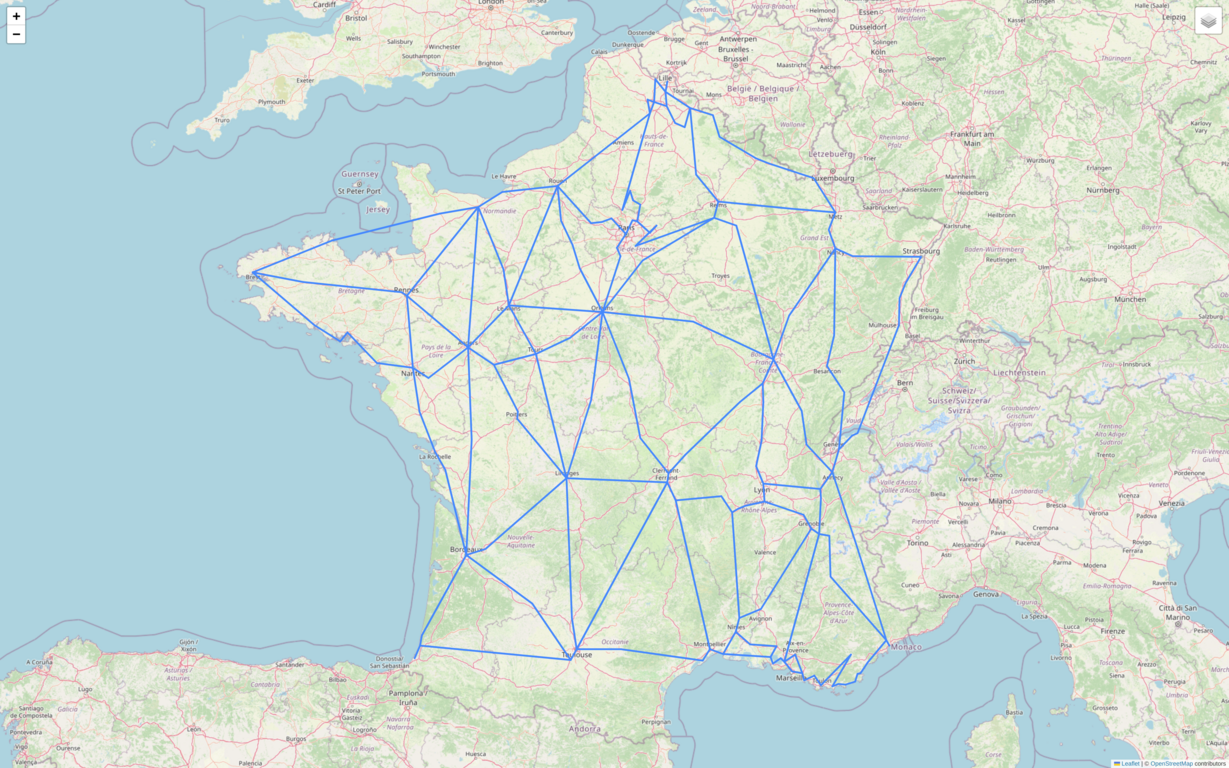
\includegraphics[height=0.6\paperheight]{images/road_detection/final graph on map.png}
        \caption{Final graph on a map (width parameter = $0.2$)}
    \end{figure}
\end{frame}

\begin{frame}{Reminder : pre-road detection thanks to the clustering methods}
    \begin{figure}
        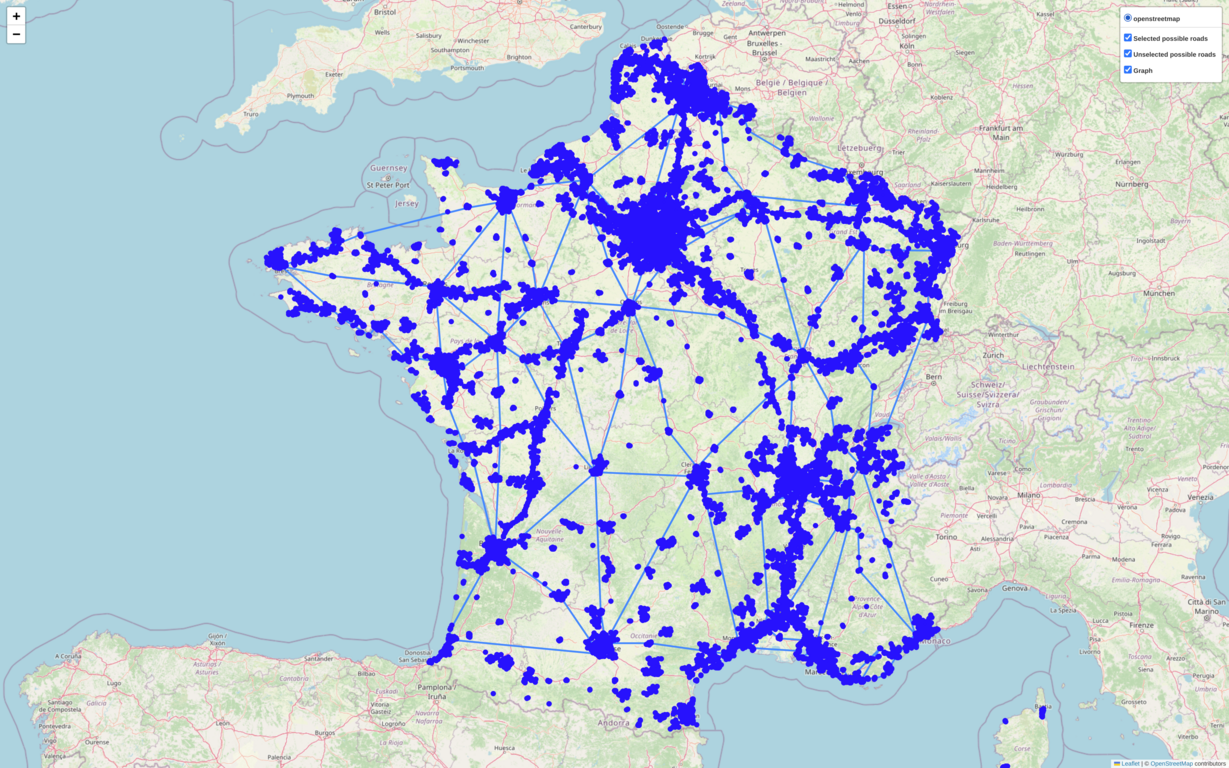
\includegraphics[height=0.6\paperheight]{images/road_detection/road-predetection and graph.png}
        \caption{Road pre-detection and graph}
    \end{figure}
\end{frame}

\begin{frame}{Final selected road base stations}
    \begin{figure}
        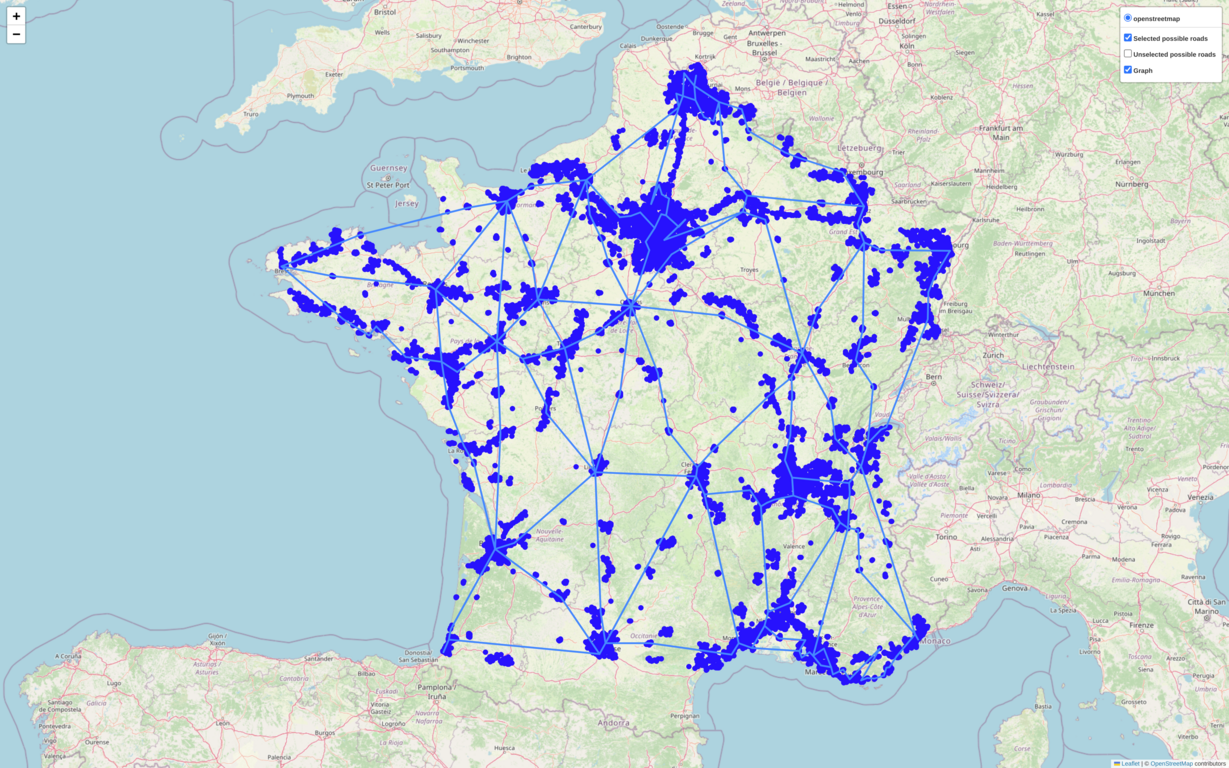
\includegraphics[height=0.6\paperheight]{images/road_detection/roads detected.png}
        \caption{Nodes detected as roads after the method}
    \end{figure}
\end{frame}